%Created on: July 8, 2014       Edited by: Wesley Kyle
%Edited on: July 22, 2014       Edited by: Shantel Butler
%Edited on:                     Edited by:
%Edited on:                     Edited by:
%Edited on:                     Edited by:
%Edited on:                     Edited by:
%Edited on:                     Edited by:
%Edited on:                     Edited by:


% This is a template for the production of all future lab documents
% 
% IMPORTANT: Edit only between the line "%%%start %%% DO NOT REMOVE THIS LINE"
% and %%%end %%% DO NOT REMOVE THIS LINE
%
% To compile the tex file use the command pdflatex

\documentclass[justified]{tufte-book}
\usepackage{graphicx} % allow embedded images
\setkeys{Gin}{width=\linewidth,totalheight=\textheight,keepaspectratio}
\usepackage{amsmath}  % extended mathematics
\usepackage{booktabs} % book-quality tables
\usepackage{units}    % non-stacked fractions and better unit spacing
\usepackage{multicol} % multiple column layout facilities
\usepackage{fancyvrb} % extended verbatim environments
\fvset{fontsize=\normalsize}% default font size for fancy-verbatim environments
\usepackage{tikz} %for drawing nice pictures
\usepackage{indentfirst}
\usepackage{enumitem}
\usepackage{fancyhdr}
\usepackage{soul}
\usepackage{marvosym}
\pagestyle{fancy}
\usepackage{float}
\allowdisplaybreaks % allows equations to span two pages if needed
\restylefloat{table}
\usetikzlibrary{arrows,snakes,shapes,calc,patterns}
\usetikzlibrary{circuits.ee.IEC}
%\usepackage[T1]{fontenc}
%\usepackage[utf8]{inputenc}

\fancyhf{} % clear all header and footer fields
\fancyfoot[C]{\footnotesize \thepage}
\renewcommand{\headrulewidth}{0pt}
\renewcommand{\footrulewidth}{0pt}


\begin{document}

\chapter{RLC Resonant Circuits - Companion Guide}

%%%start %%% DO NOT REMOVE THIS LINE

\section{Equipment}
%first column
\begin{minipage}[t]{0.6\textwidth}
\begin{itemize}[noitemsep]
\item Series and parallel RLC circuit board
\item B \& K 3011 function generator
\item set of connecting leads (2)
\end{itemize}
\end{minipage}
%second column
\begin{minipage}[t]{0.35\textwidth}
\begin{itemize}[noitemsep]
\item Oscilloscope
\end{itemize}
\end{minipage}


\section{Setup}
\begin{figure}
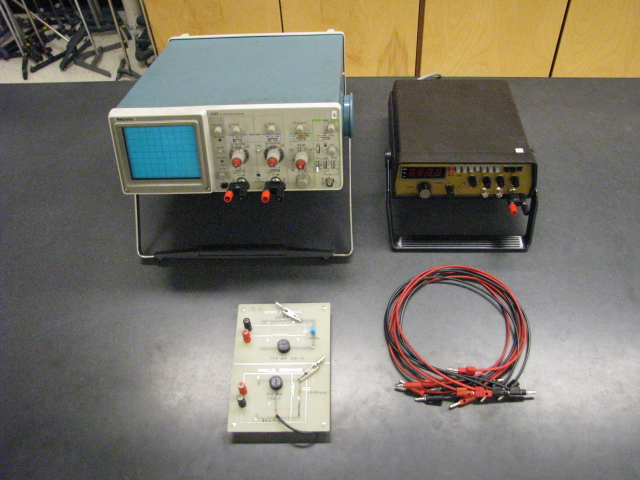
\includegraphics{RLC-Resonant-Circuits-Setup.jpg}
\caption{Equipment Setup}
\label{pic:RLCsetup}
\end{figure}

Set up bench as shown in Figure \ref{pic:RLCsetup}.

\section{Maintenance}

\begin{enumerate}
\item 
\item 
\end{enumerate}

\section{Critical Points of Failure}

There are currently no known critical points of failure.

\section{Notes to the Instructor}
\begin{enumerate}
\item The function generator outputs a dip on each node for the parallel circuit at amplitude resonant frequency. This caused difficulty in measuring the experimental amplitude resonant frequency since the output frequency could be adjusted within a 100 Hz range while still exhibiting resonant attributes on the oscilloscope. 
\item 
\item 
\end{enumerate}

\section{Prelab Questions}
\begin{enumerate}
\item Resonance is the tendency of a system to oscillate with a greater amplitude at some frequencies than at others (Wikipedia - Resonance). Four examples of physical systems that exhibit resonant qualities: musical instruments (acoustic resonance), suspension systems (mechanical resonance), electrical circuits (electrical resonance), and optical cavities (optical resonance).
\item Derivation of $\omega^2 = 1/LC$: First set $\phi=0$ in Equation 8 (the condition for phase resonance),
$$
0=tan^{-1}\left[ \frac{1}{R} \left( \omega L - \frac{1}{\omega C} \right) \right]
$$
Rearrange to get,
$$
\omega L - \frac{1}{\omega C} =0
$$
Yielding,
$$
\omega^2 = \frac{1}{LC}
$$

Then we can see that Equation 7 is at an extremum (condition for amplitude resonance) when $\omega^2 = \frac{1}{LC}$ giving
$$
E\sin\omega t = i(t)R
$$
which is the maximal current possible for the circuit. Therefore, amplitude resonance and phase resonance occur at the same frequency $\omega=1/\sqrt{LC}$.
\item Parallel phase frequency derivation: First set $\phi=0$ in Equation 13 (the condition for phase resonance) and factor $\omega$ out to get,
$$
\omega\left[\frac{\omega^2L^2C}{R}+RC-\frac{L}{R}\right]=0
$$
Rearrange to get Equation 15,
$$
\omega_P^2 = \frac{1}{LC} -\frac{R^2}{L^2}
$$
\item Justification for Equation 6 (series circuit): Substituting voltage values into Equation 1 we have,
$$
L\frac{di}{dt}+\frac{Q}{C}+iR-E\sin\omega t = 0
$$
Taking the derivative of this gives,
$$
L\frac{d^2i}{dt^2} + R\frac{di}{dt} + \frac{i}{C} - E\omega\cos\omega t = 0
$$

which is Equation 6 from the lab manual. Therefore, this equation is valid to use for a series circuit.

Justification for Equations 9, 10, and 11 (parallel circuit): Equation 9 comes from the current splitting at the node (Kirchhoff's current law) that can be seen in Figure 4. We can then treat each current, $i_1$ and $i_2$, as part of a separate circuit. Equation 10 corresponds to $i_1$ where the voltage source, inductor, and resistor are seen as one circuit. Then Kirchhoff's voltage law is applied to give Equation 10. Equation 11 corresponds to $i_2$ in the same way where just the capacitor and voltage sources are seen as the second circuit. Kirchhoff's voltage law is applied to the circuit and then the derivative is taken with respect to time to give Equation 11.
\item Setting R=0 in Equation 14 gives,
$$
\omega_A ^2 = \frac{1}{LC}
$$
Similarly for Equation 15,
$$
\omega_P ^2 = \frac{1}{LC}
$$
which implies that 
$$
\omega_A=\omega_P=\omega=\frac{1}{\sqrt{LC}}
$$
So, the resonant frequencies in the parallel circuit are equal when there is no resistance and are also equal to the resonant frequency of the series circuit.
\end{enumerate}


\section{Data Requirements}
\begin{enumerate}[resume]
\item The series circuit values were recorded to be: R=50.8 $\Omega$, C=1.00$\times$10$^{-6}$ F, L=0.474 H. When substituted into,
$$
f=\frac{1}{2\pi\sqrt{LC}}
$$
the theoretical resonant frequency was found to be f=231.17 Hz.

The parallel circuit values were recorded to be: R=3263 $\Omega$, C=9.00$\times$10$^{-9}$ F, L=0.475 H. When substituted into,
$$
f_A=\frac{1}{LC}\sqrt{1+\frac{2R^2C}{L}}-\frac{R^2}{L^2}
$$
and
$$
f_P=\frac{1}{2\pi}\sqrt{\frac{1}{LC}\sqrt{1+\frac{2R^2C}{L}}-\frac{R^2}{L^2}}
$$
the theoretical amplitude resonant frequency was found to be f$_A$=2404.49 Hz and the theoretical phase resonant frequency was found to be f$_P$=2135.10 Hz.
\item The experimental resonant frequency for the series circuit was found to be f=230$\pm$ 2 Hz. For the parallel circuit, the experimental amplitude resonant frequency was found to be f$_A$=2300$\pm$ 20 Hz and the experimental phase resonant frequency was found to be f$_P$=2000$\pm$ 20 Hz.
\item See Data Requirement 9 (asks for the same table)
\newpage
\item Table: Series Voltage vs. Frequency and Angular Frequency
\begin{table}[H]
\center
\begin{tabular}{|c|c|c|c|c|c|}
\hline
f (Hz) & $\Delta$f (Hz) & $\omega$ (rad/s) & $\Delta\omega$ (rad/s) & V (V) & $\Delta$V (V)\\
\hline
158 & 2 & 993  & 10 & 0.34 & 0.05\\
169 & 2 & 1060 & 10 & 0.39 & 0.05\\
180 & 1 & 1130 & 6  & 0.44 & 0.05\\
192 & 2 & 1210 & 10 & 0.5  & 0.05\\
200 & 2 & 1260 & 10 & 0.54 & 0.05\\
211 & 1 & 1330 & 6  & 0.59 & 0.05\\
220 & 2 & 1380 & 10 & 0.62 & 0.05\\
225 & 2 & 1410 & 10 & 0.62 & 0.05\\
230 & 2 & 1450 & 10 & 0.62 & 0.05\\
235 & 2 & 1480 & 10 & 0.62 & 0.05\\
240 & 1 & 1510 & 6  & 0.61 & 0.05\\
245 & 2 & 1540 & 10 & 0.6  & 0.05\\
247 & 1 & 1550 & 6  & 0.59 & 0.05\\
250 & 2 & 1570 & 10 & 0.58 & 0.05\\
258 & 2 & 1620 & 10 & 0.56 & 0.05\\
269 & 1 & 1690 & 6  & 0.52 & 0.05\\
284 & 1 & 1780 & 6  & 0.46 & 0.05\\
295 & 2 & 1850 & 10 & 0.43 & 0.05\\
309 & 1 & 1940 & 6  & 0.39 & 0.05\\
322 & 2 & 2020 & 10 & 0.36 & 0.05\\
\hline
\end{tabular}
\label{tbl:RLCSeries}
\caption{Series Resonant Circuit Data}
\end{table}

\item Graph: Series voltage vs. angular frequency
  \begin{figure}[h!]
    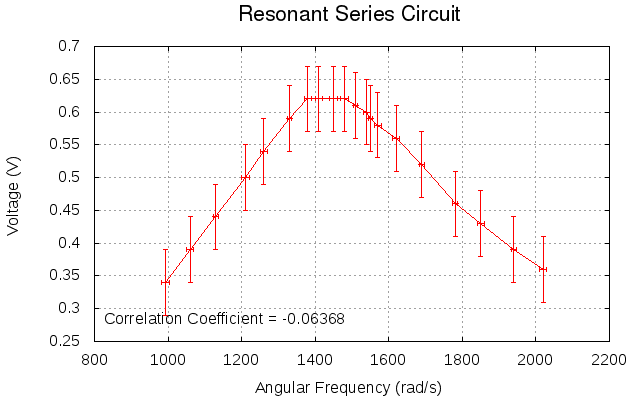
\includegraphics{RLC-Resonant-Circuits-Series-Graph.png}
    \caption{Resonant Series Circuit}
    \label{pic:RLCseries}
  \end{figure}
\item Graph: Series voltage vs. angular frequency: Experimental vs. Theoretical
  \begin{figure}[h!]
    \center
    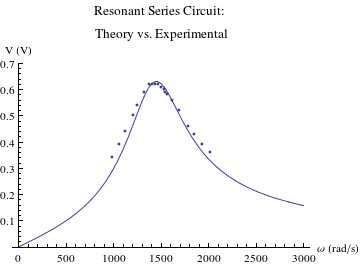
\includegraphics{RLC-Resonant-Circuits-Series-Graph-Mathematica.png}
    \caption{Resonant Series Circuit: Theoretical vs. Experimental}
    \label{pic:RLCseriesMathematica}
  \end{figure}

\newpage
\item Table: Parallel voltage vs. frequency vs. angular frequency
\begin{table}[H]
\center
\begin{tabular}{|c|c|c|c|c|c|}
\hline
f (kHz) & $\Delta$f (kHz) & $\omega$ (krad/s) & $\Delta\omega$ (krad/s) & V (V) & $\Delta$V (V)\\
\hline
1.50&0.02&9.42&0.13&8.80&1.00\\
1.60&0.01&10.1&0.06&8.00&0.50\\
1.70&0.02&10.7&0.13&7.20&0.50\\
1.80&0.02&11.3&0.13&6.30&0.50\\
1.90&0.02&11.9&0.13&5.30&0.50\\
2.00&0.02&12.6&0.13&4.30&0.50\\
2.10&0.02&13.2&0.13&2.90&0.25\\
2.20&0.02&13.8&0.13&1.75&0.25\\
2.25&0.02&14.1&0.13&1.18&0.10\\
2.30&0.02&14.5&0.13&0.94&0.10\\
2.35&0.02&14.8&0.13&0.92&0.10\\
2.40&0.02&15.1&0.13&1.40&0.10\\
2.50&0.02&15.7&0.13&2.50&0.25\\
2.60&0.02&16.3&0.13&3.50&0.25\\
2.72&0.02&17.1&0.13&4.50&0.50\\
2.80&0.02&17.6&0.13&5.20&0.50\\
2.90&0.02&18.2&0.13&5.90&0.50\\
3.00&0.02&18.8&0.13&6.50&0.50\\
3.10&0.02&19.5&0.13&7.10&0.50\\
3.20&0.02&20.1&0.13&7.50&0.50\\
\hline
\end{tabular}
\label{tbl:RLCParallel}
\caption{Parallel Resonant Circuit Data}
\end{table}
\item Graph: Parallel voltage vs. angular frequency
  \begin{figure}[h!]
    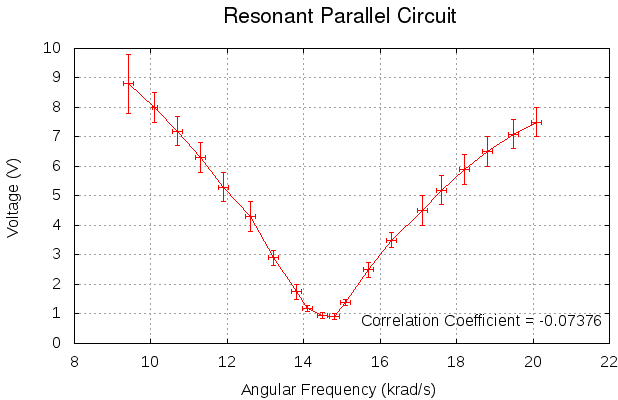
\includegraphics{RLC-Resonant-Circuits-Parallel-Graph.png}
    \caption{Resonant Parallel Circuit}
    \label{pic:RLCParallel}
  \end{figure}
\end{enumerate}


\section{Discussion}
\begin{enumerate}[resume]
\item The theoretical series resonant frequency was found to be f=231.17 Hz and the experimental value was found to be f=230$\pm$ 2 Hz. These values agree within error. 

For the parallel circuit, the theoretical amplitude resonant frequency was found to be f$_A$=2404.49 Hz and the experimental amplitude resonant frequency was found to be f$_A$=2350$\pm$ 70 Hz where the drift on the function generator occurred from 2300-2400 Hz and was accounted in the error by adding an extra 50 Hz to the original 20 Hz error inherent in the device. The theoretical phase resonant frequency was found to be f$_P$=2135.10 Hz and the experimental phase resonant frequency was found to be f$_P$=2120$\pm$ 20 Hz. Both the phase and amplitude resonant frequencies agreed within error.

Possible sources of error include: degraded devices on the circuit boards, degraded wiring, and the difficulties associated with measuring the theoretical amplitude frequency discussed in the notes below.

\textit{Notes: The function generator output exhibited a dip on each node, which made it difficult to record a proper measurement for the resonant frequencies on the parallel circuit. This error was taken into account for the amplitude resonant frequency measurement as discussed above.}
\item In Figure \ref{pic:RLCseriesMathematica}, the experimental data was plotted along with the theoretical curve. The theoretical extremum point, resonance, occurred at about 6.25 V which corresponded to the experimental resonance at $0.62\pm0.05 V$ within the error range. 
\item The results of this experiment confirm the theory of resonance, as all theoretical values matched experimental within the error range (discussed in Discussion 14).

At resonance, the current was found to be at an extremum for both the series and parallel circuits as predicted by Equations 7 and 12 from the lab manual within the experimental error range. This can be seen when values for angular frequency are substituted into Equations 7 and 12.

\end{enumerate}
%%%end %%% DO NOT REMOVE THIS LINE
\end{document}
